\section{Graph analysis}\label{GraphAnalysis}
Graph databases are part of NoSQL (also known as NotOnlySQL). They don't represent tables and relations.

There are different NoSQL databases (MariaDB, Cassandra, MarkLogic, etc...), each one is focusing on its own solution. MariaDB is document oriented, but in our case we are using Neo4j \parencite{miller2013graph} which is graph database. Instead of tables and relations, we have nodes and edges. Another change is language. Queries are not written/executed in SQL but with Cypher.

Setup of the database can be seen at \ref{A4} and data used in \ref{A5}.
%\input{Sections/GraphAnalysis/Setup/setup}

%\input{Sections/GraphAnalysis/Data/data}

\subsection{Graph 1}\label{Graph1}

First graph database is showcasing relationships between chat join, leave, mention and respond. By that we can see what chat sessions seems to be the most active.

How data was inserted can be seen in Python code bellow.
\begin{listing}[H]
\caption{User sessions -part 1}
\begin{minted}{Python}
def create_user_sessions(data_chat_join_team_chat, 
                         data_chat_leave_team_chat, 
                         data_chat_mention_team_chat, 
                         data_chat_respond_team_chat):
    uri, user, password = get_creds(0)
    driver = GraphDatabase.driver(uri, auth=(user, password))

    create_user_query = "CREATE (:User {id: $user_id})"
    create_teamchat_session_query = 
        "CREATE (:TeamchatSession {id: $teamchat_session_id, date: $date})"
    create_chat_item_query = "CREATE (:ChatItem {id: $chat_item})"
    create_chat_relation_query = 
        "MATCH (c1), (c2) WHERE 
            c1.id = $chatid1 AND 
            c2.id = $chatid2 CREATE (c1)-[:RESPONDS_TO]->(c2)"
    create_mention_relation_query = 
        "MATCH (u), (c) WHERE 
            u.id = $user_id AND 
            c.id = $chat_item CREATE (u)-[:MENTIONS]->(c)"
    create_join_relation_query = 
        "MATCH (u), (t) WHERE 
            u.id = $user_id AND 
            t.id = $teamchat_session_id CREATE (u)-[:JOINS]->(t)"
    create_leave_relation_query = 
        "MATCH (u), (t) WHERE 
            u.id = $user_id AND 
            t.id = $teamchat_session_id CREATE (u)-[:LEAVES]->(t)"
\end{minted}
\end{listing}

\begin{listing}[H]
\caption{User sessions -part 2}
\begin{minted}{Python}
    queries = [
        (create_user_query, 
            data_chat_join_team_chat.select("user_id")
            .distinct()),
        (create_teamchat_session_query, 
            data_chat_join_team_chat
            .select("teamchat_session_id", "date")
            .distinct()),
        (create_chat_item_query, 
            data_chat_mention_team_chat
            .select("chat_item")
            .distinct()),
        (create_chat_relation_query, 
            data_chat_respond_team_chat
            .select("chatid1", "chatid2")),
        (create_mention_relation_query, 
            data_chat_mention_team_chat
            .select("user_id", "chat_item")),
        (create_join_relation_query, 
            data_chat_join_team_chat
            .select("user_id", "teamchat_session_id")),
        (create_leave_relation_query, 
            data_chat_leave_team_chat
            .select("user_id", "teamchat_session_id"))
    ]

    with driver.session() as session:
        for query, data in queries:
            for row in data.collect():
                session.run(query, **row.asDict())
\end{minted}
\end{listing}

\begin{landscape}
  \begin{figure}[H]
    \includegraphics[scale=0.047]{img/Neo4j/graph0.png}
    \centering
    \caption{Graph 1}
    \label{fig:Graph 1}
  \end{figure}
\end{landscape}

If we want to filter the nodes by the most mentioned, we can use Cypher code from bellow. This will showcase top mentioned nodes and their relations.

\begin{listing}[H]
\caption{Cypher filter 1}
\begin{minted}{Cypher}
MATCH (n)-[r]->()
WHERE TYPE(r) IN ['RESPONDS_TO', 'MENTIONS', 'JOINS', 'LEAVES']
WITH n, COUNT(*) AS mentionsCount
ORDER BY mentionsCount DESC
LIMIT 10
MATCH (n)-[r]->(m)
RETURN n, r, m
\end{minted}
\end{listing}

\begin{landscape}
  \begin{figure}[H]
    \includegraphics[scale=0.18]{img/Neo4j/graph0-filter.png}
    \centering
    \caption{Graph 1 filtered}
    \label{fig:Graph 1 filtered}
  \end{figure}
\end{landscape}


\newpage
\subsection{Graph 2}\label{Graph2}

Messages between users are not as important to us as they are between the users. What is important to us is reasoning for n number of messages. If users are constantly interacting, it means that they are satisfied and would gladly return. 

Function bellow showcases how data was inserted.
\begin{listing}[H]
\caption{Messages between users -part 1}
\begin{minted}{Python}
def create_msg_between_users(data_chat_join_team_chat, 
                             data_chat_leave_team_chat, 
                             data_chat_mention_team_chat, 
                             data_chat_respond_team_chat):
    uri, user, password = get_creds(1)
    driver = GraphDatabase.driver(uri, auth=(user, password))

    create_user_query = "MERGE (:User {id: $user_id})"
    create_teamchat_session_query = 
        "MERGE (:TeamchatSession {id: $teamchat_session_id, date: $date})"
    create_chat_item_query = "MERGE (:ChatItem {id: $chat_item})"
    create_chat_relation_query = """
        MATCH (c1), (c2) 
        WHERE c1.id = $chatid1 AND c2.id = $chatid2 
        AND c1.user_id <> c2.user_id 
        CREATE (c1)-[:RESPONDS_TO]->(c2)
    """
    create_mention_relation_query = 
        "MATCH (u), (c) WHERE 
            u.id = $user_id AND 
            c.id = $chat_item CREATE (u)-[:MENTIONS]->(c)"
    create_join_relation_query = 
        "MATCH (u), (t) WHERE 
            u.id = $user_id AND 
            t.id = $teamchat_session_id CREATE (u)-[:JOINS]->(t)"
    create_leave_relation_query = 
        "MATCH (u), (t) WHERE 
            u.id = $user_id AND 
            t.id = $teamchat_session_id CREATE (u)-[:LEAVES]->(t)"
    create_send_relation_query = 
        "MATCH (u), (c), (t) WHERE 
            u.id = $user_id AND c.id = $chat_item AND 
            t.id = $teamchat_session_id CREATE (u)-[:SENDS]->(c)-[:IN]->(t)"
\end{minted}
\end{listing}

\begin{listing}[H]
\caption{Messages between users -part 2}
\begin{minted}{Python}
    queries = [
        (create_user_query, 
            data_chat_join_team_chat
            .select("user_id").distinct()),
        (create_teamchat_session_query, 
            data_chat_join_team_chat
            .select("teamchat_session_id", "date").distinct()),
        (create_chat_item_query, 
            data_chat_mention_team_chat
            .select("chat_item").distinct()),
        (create_chat_relation_query, 
            data_chat_respond_team_chat
            .select("chatid1", "chatid2")),
        (create_mention_relation_query, 
            data_chat_mention_team_chat
            .select("user_id", "chat_item")),
        (create_join_relation_query, 
            data_chat_join_team_chat
            .select("user_id", "teamchat_session_id")),
        (create_leave_relation_query, 
            data_chat_leave_team_chat
            .select("user_id", "teamchat_session_id")),
        (create_send_relation_query, 
            data_chat_mention_team_chat
            .join(data_chat_join_team_chat["user_id"])
            .join(data_chat_leave_team_chat, ["user_id", "teamchat_session_id"])
            .select("user_id", "chat_item", "teamchat_session_id"))
    ]

    with driver.session() as session:
        for query, data in queries:
            for row in data.collect():
                session.run(query, **row.asDict())
\end{minted}
\end{listing}

\begin{landscape}
    \begin{figure}[H]
        \includegraphics[scale=0.048]{img/Neo4j/graph1.png}
        \centering
        \caption{Graph 2}
        \label{fig:graph1}
    \end{figure}
\end{landscape}

If we want to see the most messages send, we can execute the code bellow in order to see what users seem to be the most active.
\begin{listing}[H]
\caption{Cypher filter 2}
\begin{minted}{Cypher}
MATCH (n)-[r:SENDS]->()
WITH n, COUNT(r) AS sendsCount
ORDER BY sendsCount DESC
LIMIT 10
MATCH (n)-[rel]->(m)
RETURN n, rel, m
\end{minted}
\end{listing}

\begin{landscape}
  \begin{figure}[H]
    \includegraphics[scale=0.15]{img/Neo4j/graph1-filter.png}
    \centering
    \caption{Cypher filter 2}
    \label{fig:Graph 2 filtered}
  \end{figure}
\end{landscape}
\newpage
\subsection{Graph 3}\label{Graph3}

This graph is a representation of all the data. The idea is to have one big graph that we could fitler information from.

Data insertion is showcased with the function bellow.
\begin{listing}[H]
\caption{Mega graph -part 1}
\begin{minted}{Python}
def create_mega_graph(mega_dataframe):
    uri, user, password = get_creds(2)
    driver = GraphDatabase.driver(uri, auth=(user, password))

    create_user_query = "MERGE (:User {id: $userId})"
    create_country_query = "MERGE (:Country {name: $country})"
    create_team_query = "MERGE (:Team {id: $teamId, name: $name})"
    create_platform_query = "MERGE (:PlatformType {name: $platformType})"
    create_ad_query = "MERGE (:Ad {id: $adId})"
    create_category_query = "MERGE (:AdCategory {name: $adCategory})"
    create_country_user_rel_query = 
        "MATCH (u:User), (c:Country) WHERE 
            u.id = $userId AND 
            c.name = $country CREATE (u)-[:BELONGS_TO_COUNTRY]->(c)"
    create_team_user_rel_query = 
        "MATCH (u:User), (t:Team) WHERE 
            u.id = $userId AND 
            t.id = $teamId CREATE (u)-[:MEMBER_OF_TEAM {strength: $strength}]->(t)"
    create_platform_user_rel_query = 
        "MATCH (u:User), (p:PlatformType) WHERE 
            u.id = $userId AND 
            p.name = $platformType CREATE (u)-[:USES_PLATFORM]->(p)"
    create_ad_user_rel_query = 
        "MATCH (u:User), (a:Ad) WHERE 
            u.id = $userId AND 
            a.id = $adId CREATE (u)-[:VIEWED_AD]->(a)"
    create_category_ad_rel_query = 
        "MATCH (a:Ad), (c:AdCategory) WHERE 
            a.id = $adId AND 
            c.name = $adCategory CREATE (a)-[:BELONGS_TO_CATEGORY]->(c)"
\end{minted}
\end{listing}

\begin{listing}[H]
\caption{Mega graph -part 2}
\begin{minted}{Python}
    queries = [
        (create_user_query, 
            mega_dataframe.select("userId")
            .distinct()),
        (create_country_query, 
            mega_dataframe.select("country")
            .distinct()),
        (create_team_query, 
            mega_dataframe
            .select("teamId", "name")
            .distinct()),
        (create_platform_query, 
            mega_dataframe
            .select("platformType")
            .distinct()),
        (create_ad_query, 
            mega_dataframe
            .select("adId")
            .distinct()),
        (create_category_query, 
            mega_dataframe
            .select("adCategory")
            .distinct()),
        (create_country_user_rel_query, 
            mega_dataframe
            .select("userId", "country")),
        (create_team_user_rel_query, 
            mega_dataframe
            .select("userId", "teamId", "strength", "name")),
        (create_platform_user_rel_query, 
            mega_dataframe
            .select("userId", "platformType")),
        (create_ad_user_rel_query, 
            mega_dataframe
            .select("userId", "adId")),
        (create_category_ad_rel_query, 
            mega_dataframe
            .select("adId", "adCategory"))
    ]

    with driver.session() as session:
        for query, data in queries:
            for row in data.collect():
                session.run(query, **row.asDict())
\end{minted}
\end{listing}

\begin{landscape}
    \begin{figure}[H]
        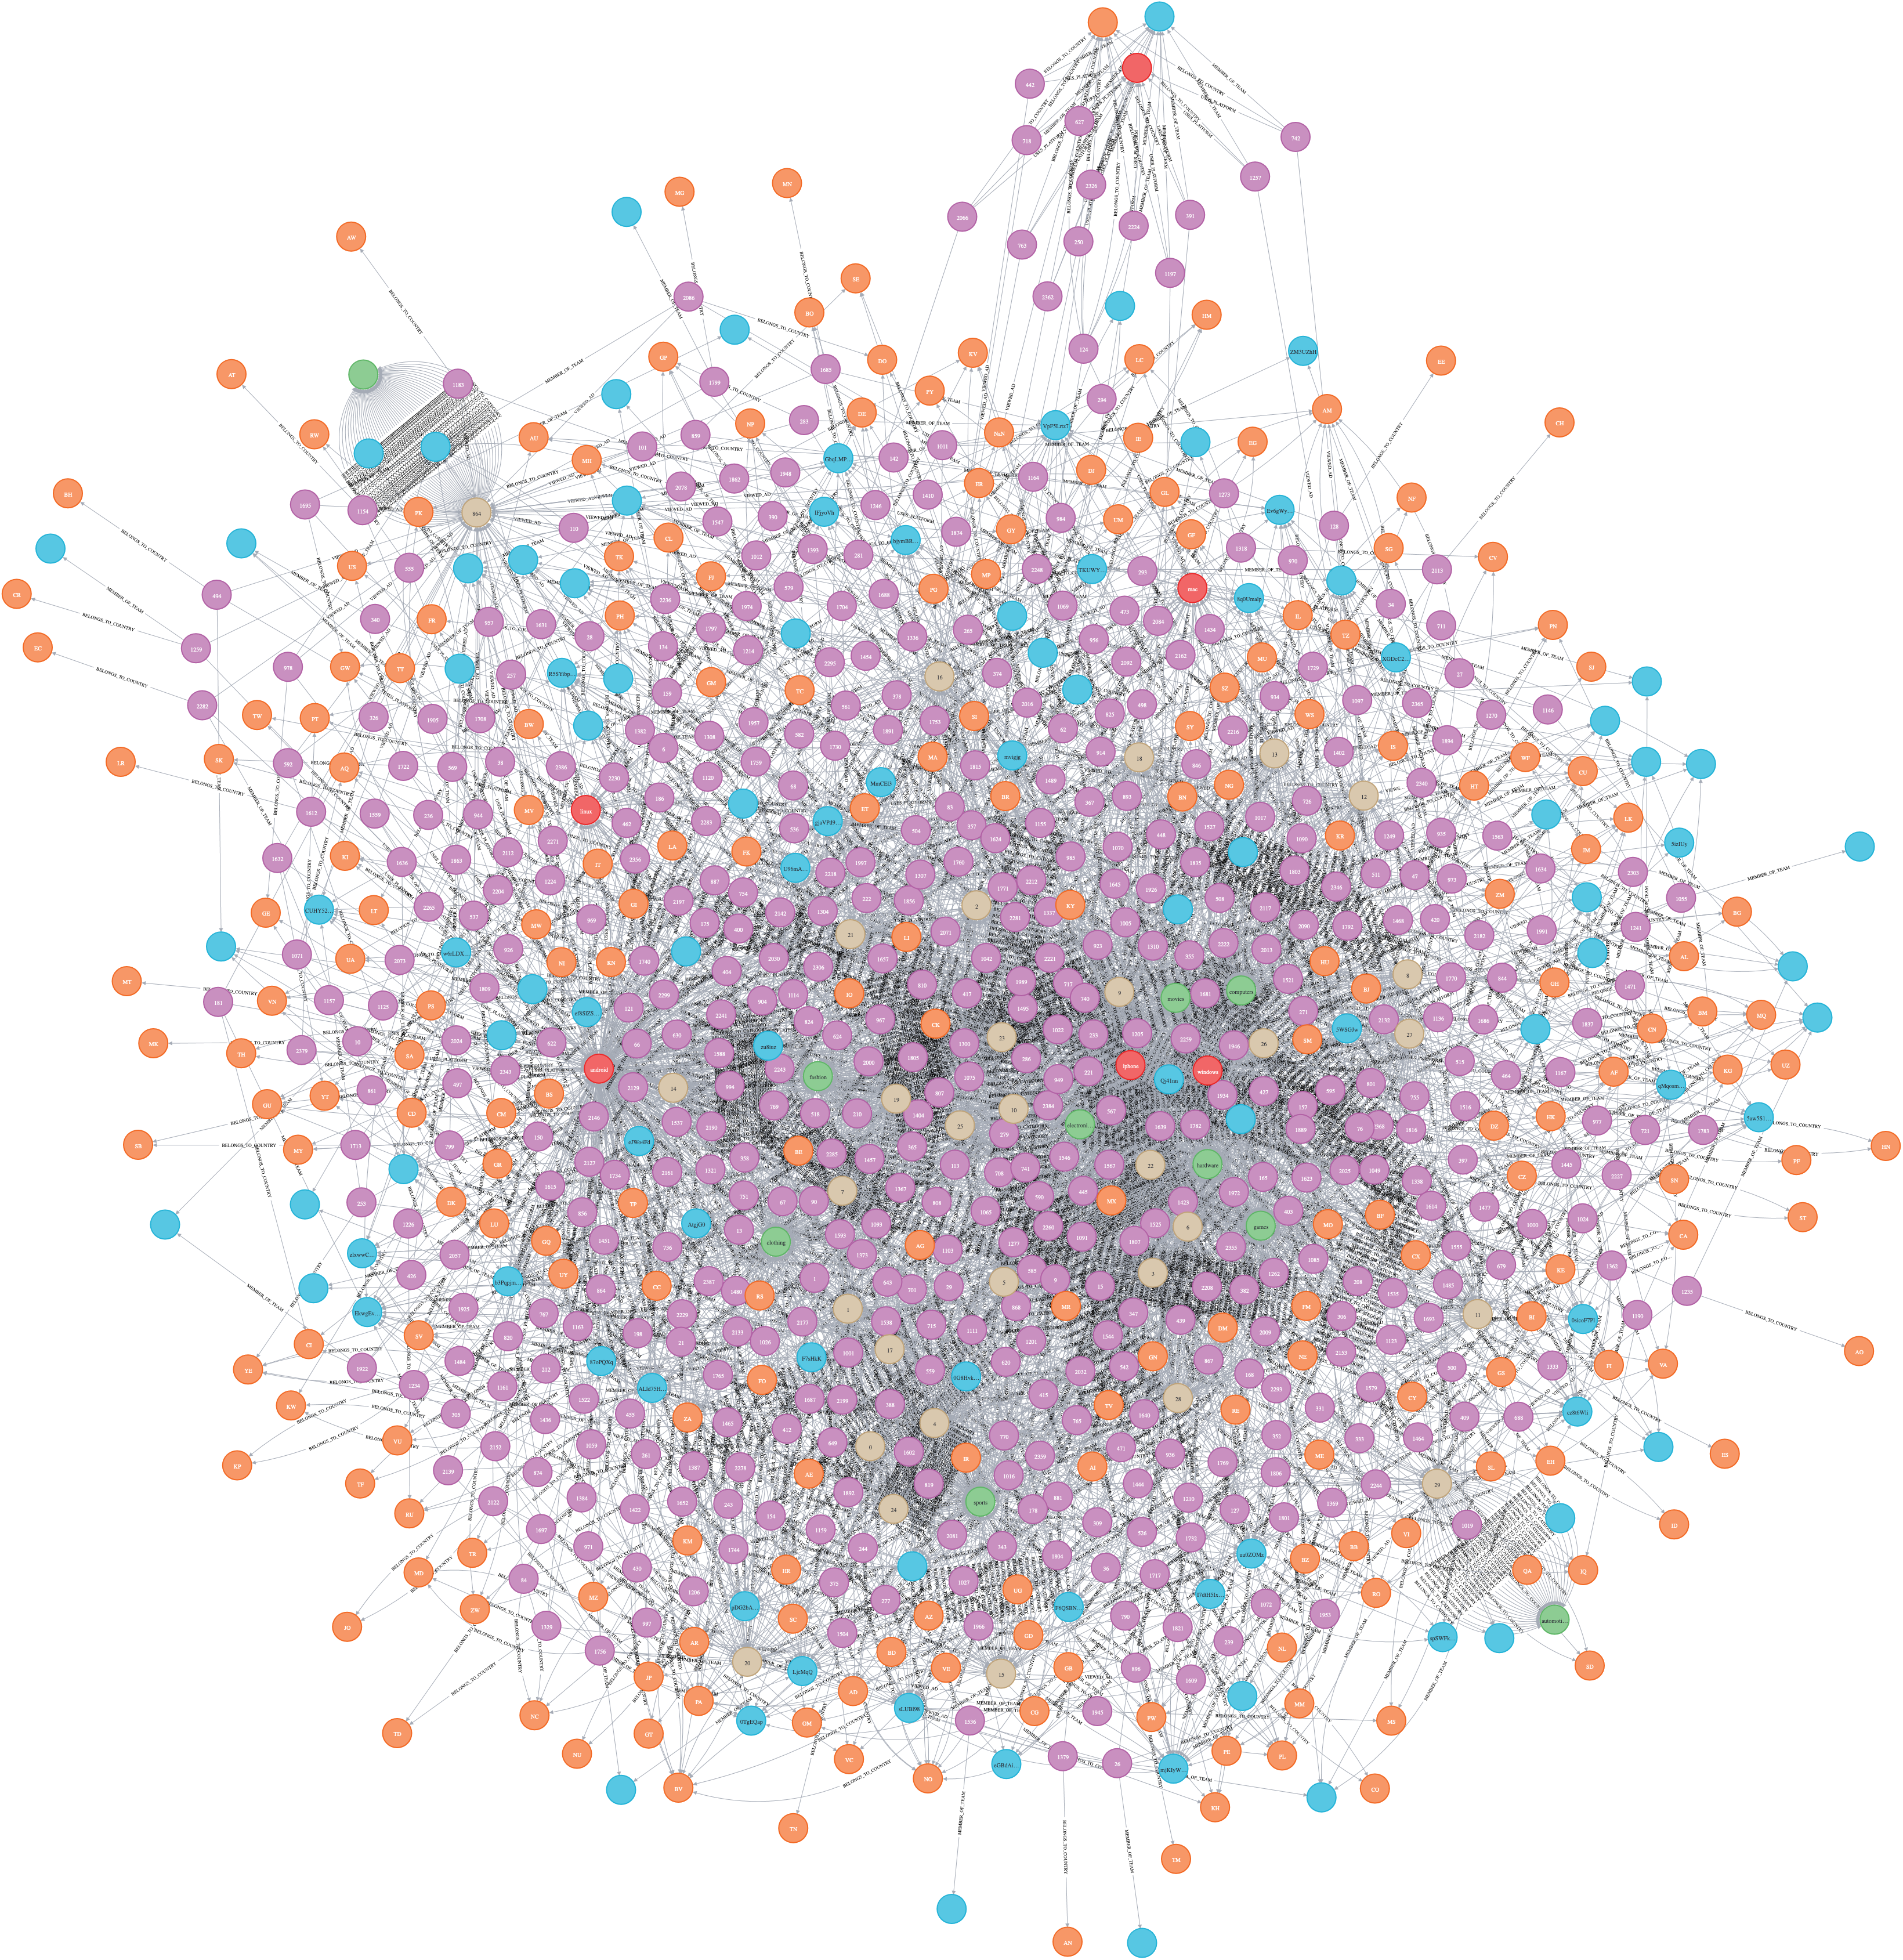
\includegraphics[scale=0.109]{img/Neo4j/graph2.png}
        \centering
        \caption{Graph 3}
        \label{fig:graph2}
    \end{figure}
\end{landscape}

We can filter out couturiers with most of the users.
\begin{listing}[H]
\caption{Cypher filter 3}
\begin{minted}{Cypher}
MATCH (n)-[r:BELONGS_TO_COUNTRY]->()
WITH n, COUNT(r) AS belongsToCountryCount
ORDER BY belongsToCountryCount DESC
LIMIT 10
MATCH (n)-[rel]->(m)
RETURN n, rel, m
\end{minted}
\end{listing}

\begin{landscape}
  \begin{figure}[H]
    \includegraphics[scale=0.37]{img/Neo4j/graph2-filter.png}
    \centering
    \caption{Graph 3 filtered}
    \label{fig:graph0}
  \end{figure}
\end{landscape}
\newpage
\subsection{Graph 4}\label{Graph4}

The final graph showcases how users are connected to ads. From marketing perspective, this could be the most important part. For example, we could see what advertisements are popular per country.

Insertion of the data is demonstrated with the function bellow.
\begin{listing}[H]
\caption{Advertisements graph -part 1}
\begin{minted}{Python}
def create_ad_graph(ad_dataframe):
    uri, user, password = get_creds(3)
    driver = GraphDatabase.driver(uri, auth=(user, password))

    create_user_query = "MERGE (:User {id: $userId})"
    create_country_query = "MERGE (:Country {name: $country})"
    create_team_query = 
        "MERGE (:Team {id: $teamId, name: $team, price: $price})"
    create_ad_query = "MERGE (:Ad {id: $adId, category: $adCategory})"
    create_user_country_relation_query = 
        "MATCH (u:User), (c:Country) WHERE 
            u.id = $userId AND 
            c.name = $country CREATE (u)-[:LIVES_IN]->(c)"
    create_user_team_relation_query = 
        "MATCH (u:User), (t:Team) WHERE 
            u.id = $userId AND 
            t.id = $teamId CREATE (u)-[:SUPPORTS]->(t)"
    create_team_ad_relation_query = 
        "MATCH (t:Team), (a:Ad) WHERE 
            t.id = $teamId AND 
            a.id = $adId CREATE (t)-[:SHOWS]->(a)"
\end{minted}
\end{listing}

\begin{listing}[H]
\caption{advertisements graph -part 2}
\begin{minted}{Python}
    queries = [
        (create_user_query, 
            ad_dataframe
            .select("userId")
            .distinct()),
        (create_country_query, 
            ad_dataframe
            .select("country")
            .distinct()),
        (create_team_query, 
            ad_dataframe
            .select("teamId", "team", "price")
            .distinct()),
        (create_ad_query, 
            ad_dataframe
            .select("adId", "adCategory")
            .distinct()),
        (create_user_country_relation_query, 
            ad_dataframe
            .select("userId", "country")),
        (create_user_team_relation_query, 
            ad_dataframe
            .select("userId", "teamId")),
        (create_team_ad_relation_query, 
            ad_dataframe
            .select("teamId", "adId"))
    ]

    with driver.session() as session:
        for query, data in queries:
            for row in data.collect():
                session.run(query, **row.asDict())
\end{minted}
\end{listing}

Filter that was applied in this case was top teams (based on users) and country they are in. With this information, query can be extended in order to see what advertisements are popular in top teams.
\begin{landscape}
    \begin{figure}[H]
        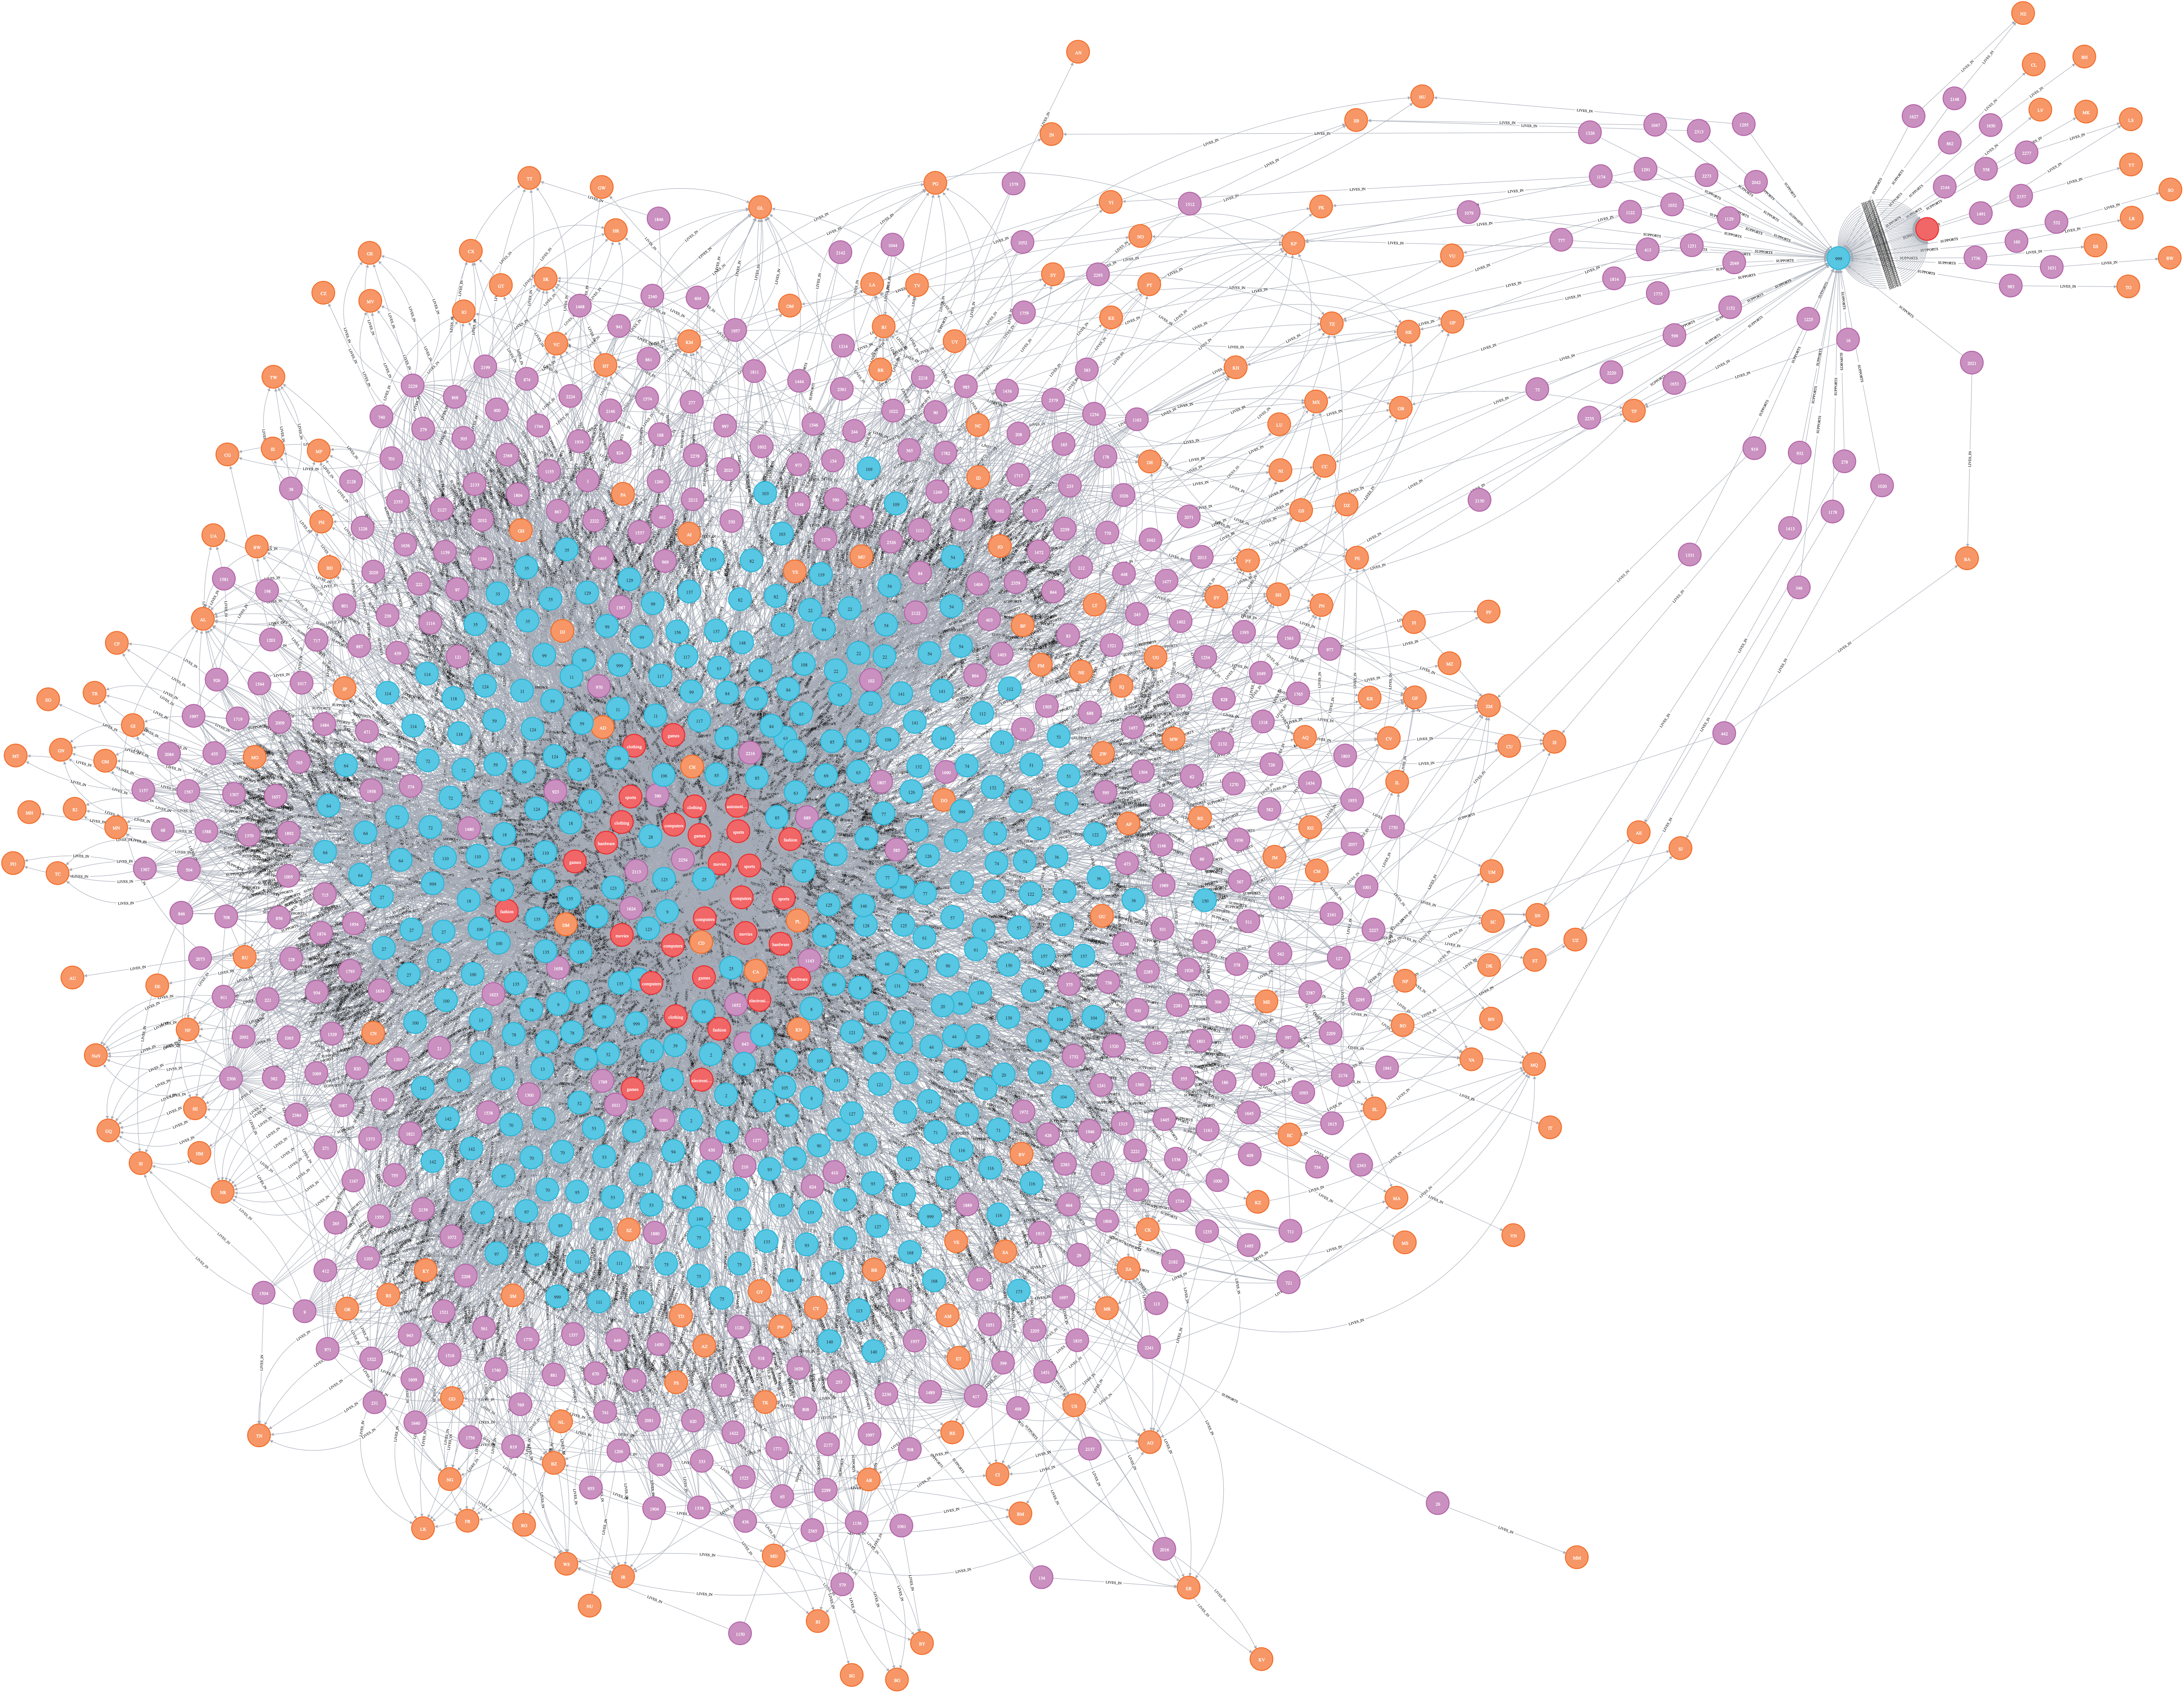
\includegraphics[scale=0.105]{img/Neo4j/graph3.png}
        \centering
        \caption{Graph 4}
        \label{fig:graph3}
    \end{figure}
\end{landscape}

\begin{listing}[H]
\caption{Cypher filter 4}
\begin{minted}{Cypher}
MATCH (n)
WHERE (n)-[:LIVES_IN|:SUPPORTS]->()
WITH n, SIZE((n)<-[:LIVES_IN|:SUPPORTS]-()) AS incomingCount
ORDER BY incomingCount DESC
LIMIT 10
MATCH (n)-[rel]->(m)
RETURN n, rel, m
\end{minted}
\end{listing}

\begin{landscape}
  \begin{figure}[H]
    \includegraphics[scale=0.25]{img/Neo4j/graph3-filter.png}
    \centering
    \caption{Graph filtered 4}
    \label{fig:graph0}
  \end{figure}
\end{landscape}
\newpage